% =====================================================================
%  MSACL DS301 Deep Learning · Lab 1 · Google Colab Setup Sheet
%  Step-by-step, with annotated screenshots of the real Colab interface.
%  Style matches labs/handouts/lab01_hints.tex (article/fancyhdr).
%
%  Screenshots live in labs/handouts/img/ and are captured from the live
%  signed-out Colab UI (see course_plan/DECISIONS.md, 2026-09-22). Re-capture
%  them when Google restyles Colab; the callout numbers are drawn on by
%  tools/make_colab_shots.py so the crops stay reproducible.
% =====================================================================
\documentclass[11pt]{article}

\usepackage[letterpaper, margin=0.55in, top=0.55in, bottom=0.45in]{geometry}
\usepackage{amsmath, amssymb}
\usepackage{xcolor}
\usepackage{fancyhdr}
\usepackage{enumitem}
\usepackage{graphicx}
\usepackage[hidelinks]{hyperref}

\definecolor{teal}{RGB}{14,124,123}
\definecolor{amber}{RGB}{224,158,47}
\definecolor{ink}{RGB}{27,32,37}

\pagestyle{fancy}
\fancyhf{}
\fancyhead[L]{\small\textbf{MSACL DS301 --- Deep Learning}}
\fancyhead[R]{\small\textbf{Lab 1: Setting up Google Colab}}
\fancyfoot[C]{\thepage}
\renewcommand{\headrulewidth}{0.4pt}

\setlength{\parindent}{0pt}
\setlength{\parskip}{2pt}
\setlist[enumerate]{leftmargin=1.6em, itemsep=1pt, topsep=1pt, parsep=0pt}
\setlist[itemize]{leftmargin=1.5em, itemsep=0pt, topsep=1pt, parsep=0pt}

% a numbered callout marker matching the circles drawn on the screenshots
\newcommand{\mk}[2][teal]{{\color{#1}\textbf{(#2)}}}
\newcommand{\step}[1]{\vspace{3pt}\textbf{\large #1}\par\vspace{1pt}}

\begin{document}
\small

\begin{center}
{\Large \textbf{Lab 1 --- Setting up Google Colab}}\\[2pt]
{\normalsize Everything runs in your browser. Nothing to install.}
\end{center}

\vspace{-1pt}
\begin{center}
\fbox{\parbox{0.95\textwidth}{\small
\textbf{What you need:} a web browser and a \textbf{free Google account}
(a personal \texttt{@gmail.com} is fine --- some hospital and university accounts
block Colab, so if yours does, use a personal one).
\textbf{You do not need:} Python, PyTorch, an install, or a GPU.
\emph{Colab} is a free Google service that runs Python notebooks on Google's
computers; your laptop only shows the page.
}}
\end{center}

\vspace{4pt}\hrule\vspace{5pt}

\step{Step 1 --- Open the Lab 1 notebook}
Click the Lab 1 link (on the course page, or type it in). It opens Colab with the
notebook already loaded --- there is nothing to download first.

\newcommand{\nburl}{https://colab.research.google.com/github/indigobio/msacl_dl_course/blob/main/student_pack/labs/lab01_training_loop.ipynb}
{\footnotesize\href{\nburl}{\color{teal}\texttt{https://colab.research.google.com/github/indigobio/msacl\_dl\_course/}\\
\phantom{xx}\texttt{blob/main/student\_pack/labs/lab01\_training\_loop.ipynb}}}

\vspace{3pt}
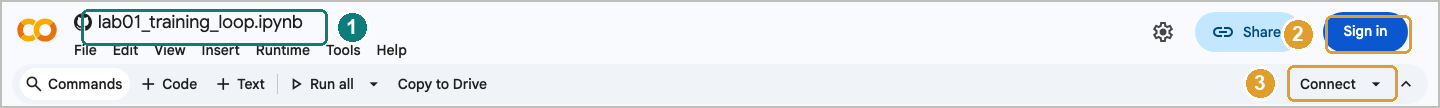
\includegraphics[width=\textwidth]{img/colab_step1_chrome.png}

\vspace{2pt}
\begin{itemize}
  \item \mk{1} Check the file name reads \texttt{lab01\_training\_loop.ipynb} --- that is the right notebook.
  \item \mk[amber]{2} \textbf{Sign in} (top right) with your Google account. Until you do, you can read the notebook but not run it.
  \item \mk[amber]{3} \textbf{Connect} (top right) starts your free machine. It usually connects on its own the first time you run a cell; if it says \emph{Connect}, click it and wait for a green tick.
\end{itemize}

\step{Step 2 --- Save your own copy \textnormal{(do this before you type anything)}}
The link opens a \emph{read-only} copy. Use \textbf{File $\rightarrow$ Save a copy in Drive}
and work in that copy, or your edits will be lost when you close the tab.
Colab opens the copy in a new tab, named \texttt{Copy of lab01\_training\_loop.ipynb} ---
\textbf{that is the tab you want to work in}.

\vspace{3pt}
\begin{center}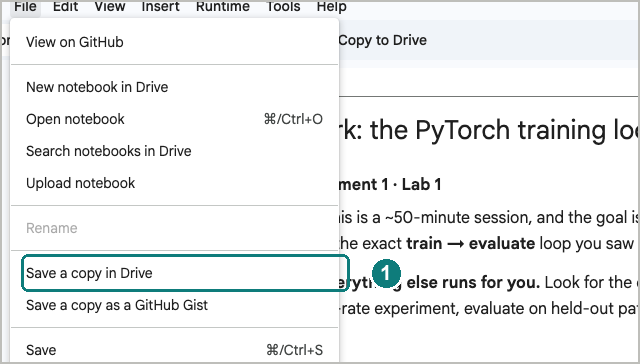
\includegraphics[width=0.50\textwidth]{img/colab_step2_savecopy.png}\end{center}

\step{Step 3 --- Run a cell}
A notebook is a list of \emph{cells}. A cell holds either text or code.
Click a code cell, then press \textbf{Shift + Enter} --- or hover over the
\mk{1} bracket at its left, which turns into a \textbf{$\blacktriangleright$} button, and click it.

\vspace{3pt}
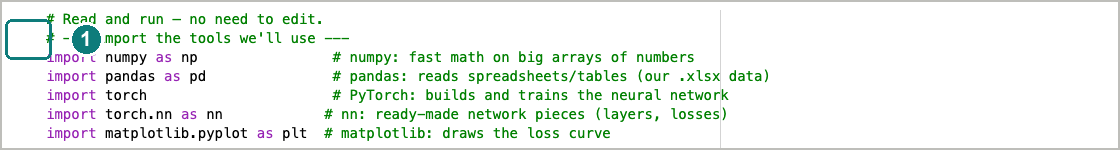
\includegraphics[width=\textwidth]{img/colab_step4_cell.png}

\vspace{2pt}
\begin{itemize}
  \item Run the cells \textbf{in order, top to bottom}. Later cells depend on earlier ones.
  \item While a cell runs the bracket shows a spinner; when it finishes you get a number, e.g. \texttt{[1]}.
  \item \textbf{Run the first code cell, ``Setup'', before anything else.} It installs the course
        packages and downloads the lab's data for you --- about a minute, ending with
        \texttt{lab01 is ready}. You never download or copy data files yourself.
  \item Only the cells marked \textbf{YOUR TURN} (the pencil icon) need editing. Run all the others exactly as they are.
\end{itemize}

\newpage

\step{Step 4 --- If something gets tangled}
The \textbf{Runtime} menu is the fix for almost everything.

\vspace{3pt}
\begin{center}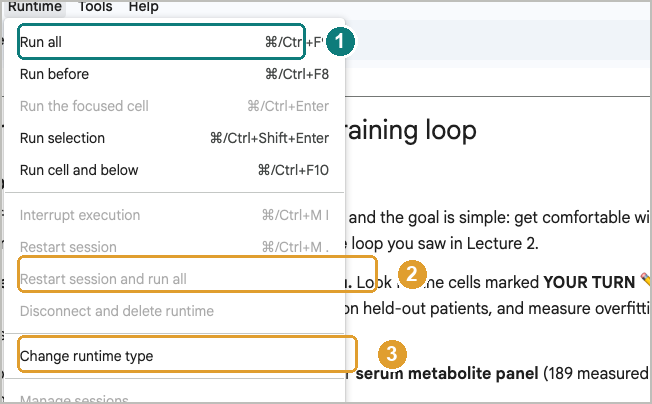
\includegraphics[width=0.54\textwidth]{img/colab_step3_runtime.png}\end{center}

\vspace{2pt}
\begin{itemize}
  \item \mk{1} \textbf{Run all} --- runs the whole notebook from the top. Good after you fix a cell.
  \item \mk[amber]{2} \textbf{Restart session and run all} --- throws away every variable and starts clean.
        This is the answer to ``it worked a minute ago''. You lose nothing but the running state; your typed code stays.
  \item \mk[amber]{3} \textbf{Change runtime type} --- where you would pick a \textbf{T4 GPU}.
        \textbf{Lab 1 does not need one}; the default CPU is plenty and connects faster. You will use this in Lab 2.
\end{itemize}

\step{Step 5 --- If the link does not open}
Go to \href{https://colab.research.google.com/}{\color{teal}\texttt{colab.research.google.com}} directly, sign in \mk[amber]{1}, then use
\textbf{File $\rightarrow$ Open notebook $\rightarrow$ GitHub} and paste
\texttt{indigobio/msacl\_dl\_course}. Or use \textbf{Upload notebook} \mk{2} if an
instructor hands you the \texttt{.ipynb} file on a USB stick.

\vspace{3pt}
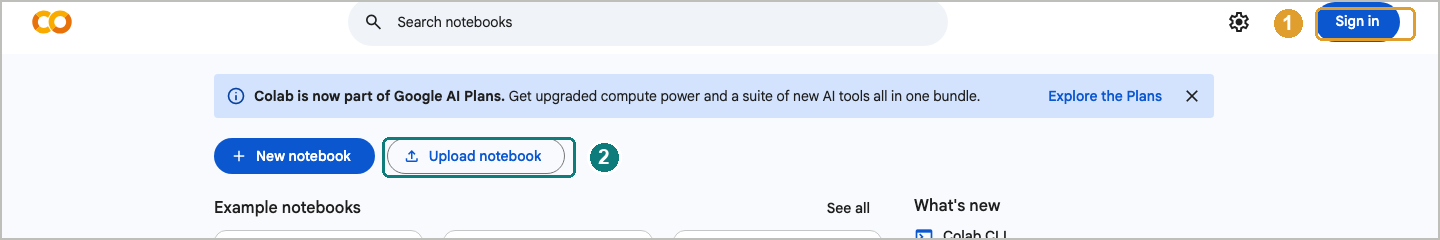
\includegraphics[width=\textwidth]{img/colab_step5_landing.png}

\vspace{5pt}\hrule\vspace{4pt}

\noindent\begin{minipage}{\textwidth}
\textbf{\large When things go wrong}

\vspace{2pt}
\begin{tabular}{@{}p{0.40\textwidth}p{0.56\textwidth}@{}}
\textbf{What you see} & \textbf{What to do} \\[2pt]
\hline\\[-6pt]
``Sign in'' keeps reappearing, or Colab will not load &
  Your institutional Google account may block Colab. Sign in with a personal
  \texttt{@gmail.com} instead. \\[3pt]
\texttt{NameError} / \texttt{... is not defined} &
  You skipped a cell, or ran them out of order. \textbf{Runtime $\rightarrow$ Restart session and run all}. \\[3pt]
A cell has been running for minutes &
  Normal for training cells. If it is stuck, \textbf{Runtime $\rightarrow$ Interrupt execution}, then restart and run all. \\[3pt]
``Cannot connect to runtime'' / disconnected &
  Free Colab disconnects after a while idle. Click \textbf{Connect} and
  \textbf{Runtime $\rightarrow$ Run all}; you lose only the running state. \\[3pt]
An \texttt{assert} cell failed &
  That is the notebook checking your answer --- it is meant to catch you.
  Read the message, fix the marked line, re-run that cell. The
  \textbf{Code Hint Sheet} lists the options for every blank. \\[3pt]
You edited the wrong tab and lost your work &
  You were in the read-only original. Redo \textbf{File $\rightarrow$ Save a copy in Drive}
  and check the tab title starts with \texttt{Copy of}. \\
\end{tabular}
\end{minipage}

\vspace{6pt}\hrule\vspace{3pt}
{\scriptsize\itshape
Screenshots are of the Google Colab interface, captured 22 September 2026, with
callout numbers added for this sheet. Colab is a Google product and its
appearance changes from time to time --- if a button has moved, the menu path in
the text is still the one to follow. A clickable version of this sheet is
\texttt{lab01\_colab\_setup.html}.}

\end{document}
